%----------------------------------------------------------------------------------------
%	PACKAGES AND OTHER DOCUMENT CONFIGURATIONS
%----------------------------------------------------------------------------------------

\documentclass[11pt,twoside,twocolumn,russian,a4paper]{article}

\usepackage{blindtext} % Package to generate dummy text throughout this template 
\usepackage{graphicx}
\usepackage{bm}
\usepackage{amsmath}
%\usepackage[sc]{mathpazo} % Use the Palatino font
\usepackage[T1,T2A]{fontenc} % Use 8-bit encoding that has 256 glyphs
\usepackage[utf8]{inputenc}
\linespread{1.05}         % Line spacing - Palatino needs more space between lines
%\usepackage{microtype}    % Slightly tweak font spacing for aesthetics

\usepackage[russian]{babel} % Language hyphenation and typographical rules

\usepackage[hmarginratio=1:1,top=32mm,bottom=32mm,left=25mm,right=25mm,columnsep=20pt]{geometry}  % Document margins
\usepackage[hang,small,labelfont=bf,up,textfont=it,up]{caption} % Custom captions under/above floats in tables or figures
\usepackage{booktabs} % Horizontal rules in tables

%usepackage{lettrine}        % The lettrine is the first enlarged letter at the beginning of the text
\usepackage{enumitem}        % Customized lists
\setlist[itemize]{noitemsep} % Make itemize lists more compact

\usepackage{abstract} % Allows abstract customization
\renewcommand{\abstractnamefont}{\normalfont\bfseries} % Set the "Abstract" text to bold
\renewcommand{\abstracttextfont}{\normalfont\small\itshape} % Set the abstract itself to small italic text

\usepackage{titlesec} % Allows customization of titles
\renewcommand\thesection{\Roman{section}} % Roman numerals for the sections
\renewcommand\thesubsection{\roman{subsection}} % roman numerals for subsections
\titleformat{\section}[block]{\large\scshape\centering}{\thesection.}{1em}{} % Change the look of the section titles
\titleformat{\subsection}[block]{\large}{\thesubsection.}{1em}{} % Change the look of the section titles

\usepackage{fancyhdr} % Headers and footers
\pagestyle{fancy}     % All pages have headers and footers
\fancyhead{}          % Blank out the default header
\fancyfoot{}          % Blank out the default footer
\fancyhead[C]{Моделирование популяции $\bullet$ Май 2018 $\bullet$ Использование приложения} % Custom header text
\fancyfoot[CO,CE]{\thepage} % Custom footer text[RO,LE]

\usepackage{titling}        % Customizing the title section
\usepackage{hyperref}       % For hyperlinks in the PDF
\usepackage{xcolor}

%----------------------------------------------------------------------------------------
%	TITLE SECTION
%----------------------------------------------------------------------------------------

\setlength{\droptitle}{-5\baselineskip} % Move the title up

\pretitle{\begin{center}\huge\bfseries} % Article title formatting
\posttitle{\end{center}} % Article title closing formatting
\title{\normalfont\color{blue} Использование приложения PopulationModeling} % Article title
\author{
	\textsc{Ф. Сергеев, В. Аксёнов} \\[0.5ex] % Your name
	\normalsize 675гр. ФУПМ МФТИ \\ % Your institution
	\normalsize \href{mailto:sergeev.fi@phystech.edu}{sergeev.fi@phystech.edu}, \href{mailto:viviaxenov@gmail.com}{viviaxenov@gmail.com}	\normalsize 
}
\date{\today} % Leave empty to omit a date

\renewcommand{\maketitlehookd}{%
\begin{abstract}
\noindent В данном документе подробно описана процедура эксплуатации приложения PopulationModeling, доступного на следующем репозитории: \color{blue}\href{https://github.com/TheodorSergeev/PopulationModeling}{github.com/TheodorSergeev/PopulationModeling} \color{black}.
\end{abstract}
}

\graphicspath{ {help-images/} }

\begin{document}

\maketitle

\section{\color{blue}Сборка и запуск}

В корневой папке находятся файлы <<Makefile.mac>>, <<Makefile.unix>> и <<Makefile.windows>>. Запустите с помощью программы \textit{make} подходящий для Вашей системы файл. Исполняемый файл будет доступен в папке \textit{/bin/Release/}. Запустите его.\smallskip\\
Альтернативно вы можете открыть и скомпилировать проектный файл <<pop-mod.cbp>> с помощью программы \color{blue}\href{http://www.codeblocks.org/}{\textit{Code::Blocks}}\color{black} или любого другого IDE, способного обрабатывать проекты \textit{Code::Blocks}.

\section{\color{blue}Выбор файла для записи статистики}

При запуске перед вами появятся несколько диалоговых окон.\\

\begin{center}
\captionsetup{type=figure}
  	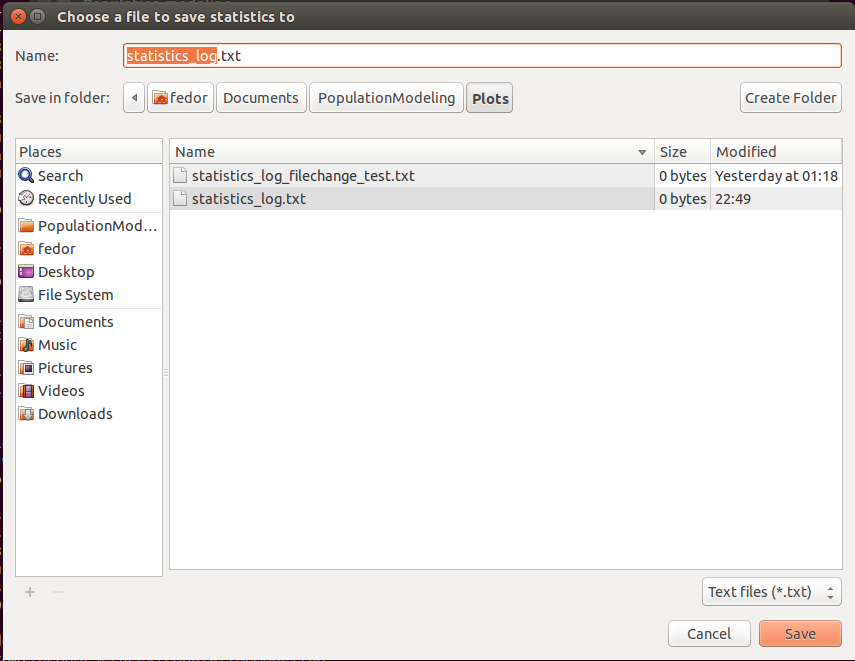
\includegraphics[width=0.4\textwidth]{help-scr2.png}
	\caption{Диалоговое окно~---~выбор файла для записи статистики по-умолчанию}
\end{center}

\noindent Первое диалоговое окно (Рис. 1) предлагает Вам использовать файл для записи статистики по умолчанию. Если Вы не хотите использовать собственный файл для записи статистики (т.~е. нажимаете No), и файл по-умолчанию доступен, то Вы переходите в следующий пункт (см. III).\smallskip\\
В случае, если Вы хотите использовать собственный файл для записи статистики (или файл по-умолчанию не может быть открыть), то перед Вами появится следующее диалоговое окно (Рис. 2). От Вас требуется выбрать Ваш файл. После выбора перед Вами появится окно (Рис. 3) для подтверждения сделанного выбора (файл будет перезаписан). Нажмите \textit{Replace}, если Вы уверенны в своём выборе.

\begin{center}
\captionsetup{type=figure}
  	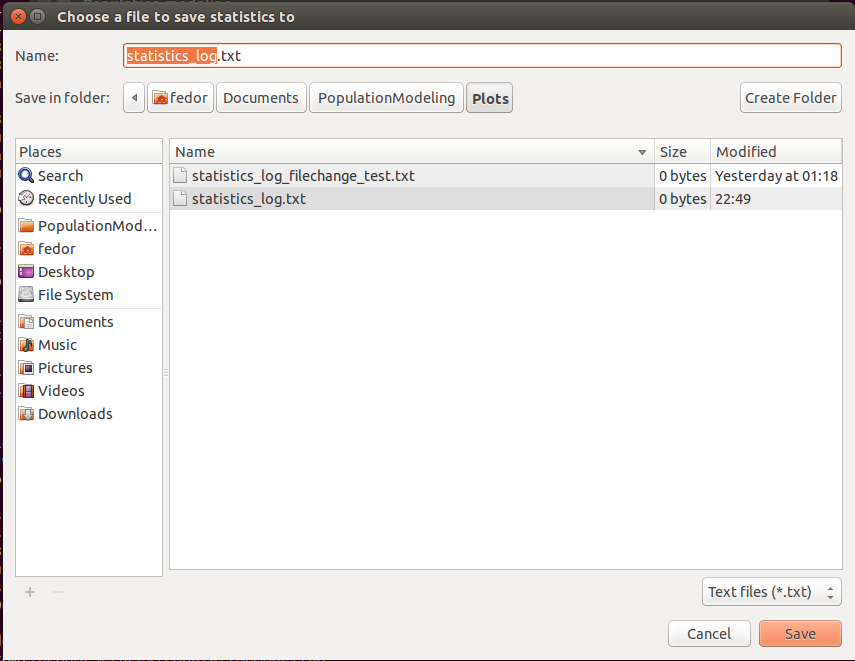
\includegraphics[width=0.4\textwidth]{help-scr2.png}
	\caption{Диалоговое окно~---~выбор собственного файла для записи статистики}
\end{center}

\begin{center}
\captionsetup{type=figure}
  	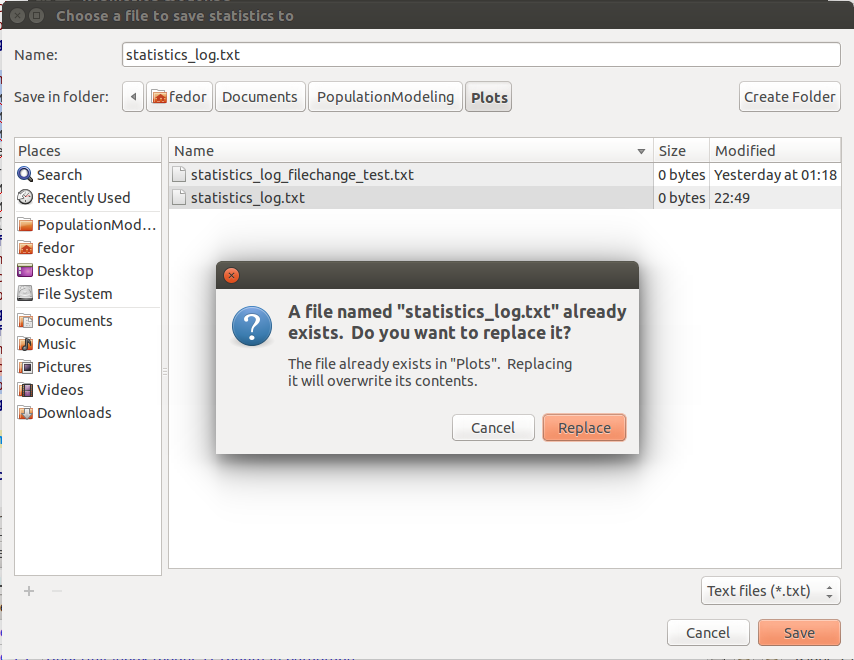
\includegraphics[width=0.4\textwidth]{help-scr3.png}
	\caption{Диалоговое окно~---~подтверждение выбора файла для записи статистики}
\end{center}

В случае, если файл не может быть открыт, Вы вернётесь на первое диалоговое окно (Рис. 1).

\section{\color{blue}Выбор файла с начальными параметрами эксперимента}

Следующим шагом является выбор файла с начальными параметрами экмперимента. Процедура аналогична выбору файла для записи статистики: сначала Вам будет предложено испольование файла по-умолчанию (Рис. 4), далее, если Вы хотите использовать свой~---~окно выбора файла (Рис. 5). В случае, если выбранный файл не может быть прочитан, Вам будет предложено выбрать другой или закрыть программу (Рис. 6). При выборе первого варианта снова откроется первое диалоговое окно (Рис 4.).

\begin{center}
\captionsetup{type=figure}
  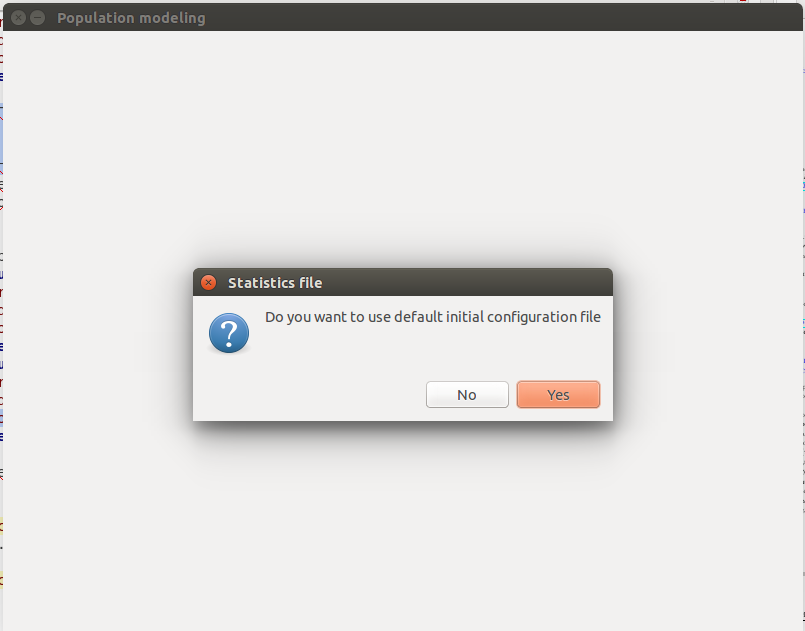
\includegraphics[width=0.4\textwidth]{help-scr4.png}
	\caption{Диалоговое окно~---~выбора файла с начальными параметрами эксперимента}
\end{center}

\begin{center}
\captionsetup{type=figure}
  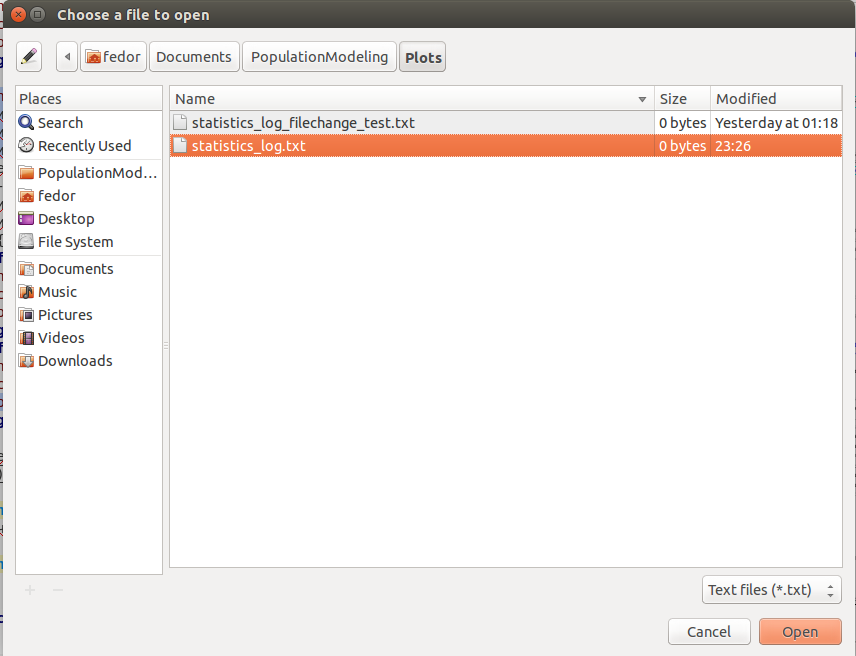
\includegraphics[width=0.4\textwidth]{help-scr5.png}
	\caption{Диалоговое окно~---~подтверждение выбора файла с начальными параметрами эксперимента}
\end{center}

\begin{center}
\captionsetup{type=figure}
  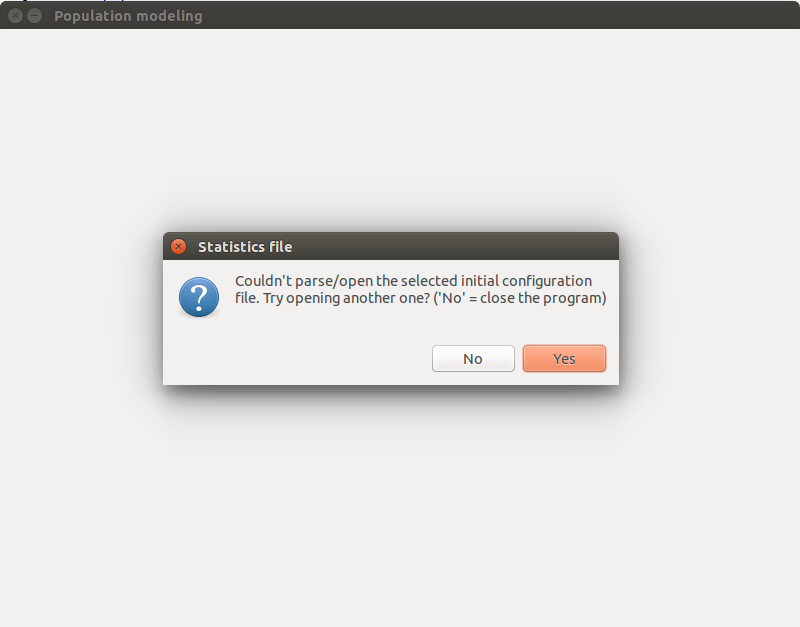
\includegraphics[width=0.4\textwidth]{help-scr6.png}
	\caption{Диалоговое окно~---~ошибка открытия файла с начальными параметрами эксперимента}
\end{center}

\section{\color{blue} Главное окно приложения}

\noindent Справа вверху три кнопки. В порядке слево направо: замедление итерации (250 мс), пауза/возобновление, ускорение итерации. Над кнопками отображается за какое время проводится одна итерация, или отображается, что эксперимент приостановлен.

\begin{center}
\captionsetup{type=figure}
  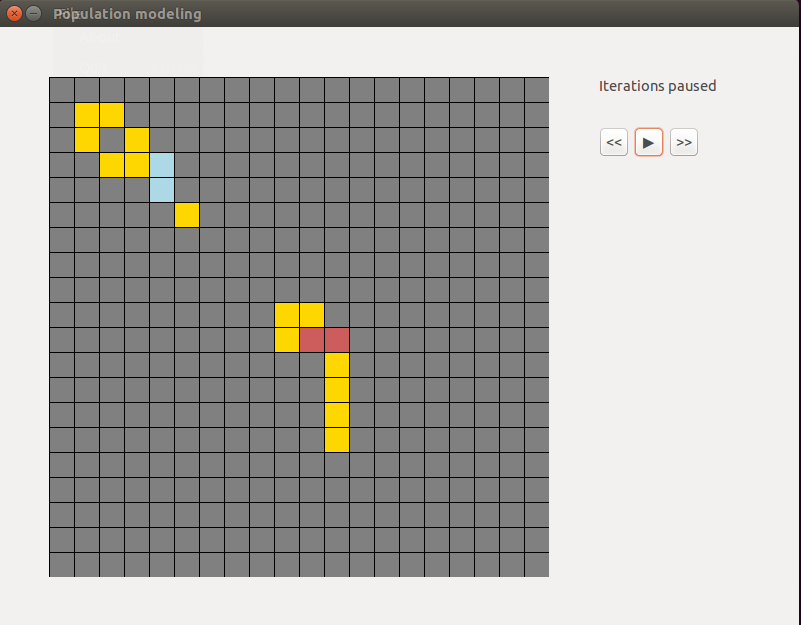
\includegraphics[width=0.4\textwidth]{help-scr8.png}
	\caption{Окно приложения}
\end{center}

\noindent В пункте верхнего меню \textit{File}: \textit{About} техническая информация о приложении, \textit{Quit}~---~закрытие приложения.\medskip\\
Посередине окна располагается поле эксперимента. Серым изображены пустые клетки, жёлтым~---~клетки еды, красным~---~первая колония бактерий, синим~---~вторая.

\section{\color{blue}Заполнение файла с начальными параметрами эксперимента}

Файл начинается со слова <<$one$>> на первой строчке, после него идёт описание первой колонии: вторая строчка $(hp,sp,rng)$, где $hp$~---~величина здоровья бактерии, $sp$~---~её скорость, $rng$~---~поле зрения (т.~е. в насколько далёкой клетке бактерия может определить содержимое). На следующей строке количество бактерий в начале эксперимента. После этого координаты $(x,y)$~---~координаты бактерии ($x$ по горизонтали, начало отсчёта~---~левый верхний угол). Аналогично для второй колонии. Только её описание начинается со слова <<$two$>>.\smallskip\\
\noindent После описания колоний стоит слово <<$start:$>>~---~мы переходим к описанию клеток пищи. На следующей строчке два числа $(N, HP)$: $N$~---~количество клеток с едой в начале эксперимента, $HP$~---~количество единиц здоровья, которое получает бактерия, поглотившая пищу. После этого для каждой из $N$ клеток идут их координаты $(x,y)$ (аналогично координатам бактерий).\smallskip\\
\noindent На следующей строке пишем слово <<$rand:$>>~---~описание закона появления пищи. Это три числа $(R, HP', T)$: $T$~---~период (количество итераций), через который появляется еда, $R$~---~количество клеток пищи, появляющееся каждый ход, $HP'$~---~количество единиц здоровья, которое получает бактерия, поглотившая пищу, для каждой из появившихся клеток.\smallskip\\
\noindent Заметим, что блоки $one$ и $two$ являются обязательными, в то время, как из блоков $start$ и $rand$ может быть указан один, оба, или ни один.

\begin{center}
\captionsetup{type=figure}
  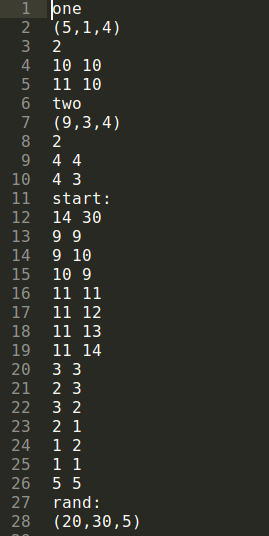
\includegraphics[width=0.2\textwidth]{help-scr9.png}
	\caption{Пример файла с начальными параметрами эксперимента}
\end{center}

\end{document}
